\documentclass[10pt]{beamer}

\usepackage[utf8]{inputenc}
\usepackage[swedish, english]{babel}
\usepackage{epstopdf}
\epstopdfsetup{update} % only regenerate pdf files when eps file is newer
\usepackage[squaren]{SIunits}
\usepackage{subfig}

\usetheme[progressbar=frametitle]{metropolis}

\usepackage{booktabs}
\usepackage[scale=2]{ccicons}

\usepackage{pgfplots}
\usepgfplotslibrary{dateplot}

\usepackage{xspace}
\newcommand{\themename}{\textbf{\textsc{metropolis}}\xspace}

\usepackage{media9}

%\setbeamertemplate{frame footer}{Niklas Ericson - Linköping University}
\setbeamercolor{progress bar}{ fg = CERNBlue , bg = CERNBlue!30 }
\setbeamercolor{alerted text}{ fg = CERNBlue , bg = CERNBlue!30 }

\title{Presentation of Master's Thesis}
\subtitle{Investigation of Control Approaches for a High Precision, \\ Piezo-actuated Rotational Stage}
\date{\today}
\author{Niklas Ericson}
\institute{Linköping University | European Organization for Nuclear Research}
\titlegraphic{\hfill
\includegraphics[height=1cm, trim=0cm 0.65cm 0cm 0cm, clip=true]{../fig/LiU_primary_black}
              \hspace{0.2cm}
\includegraphics[height=1.2cm]{../fig/CERNLogoBadge}}

\begin{document}

\maketitle

\begin{frame}{Table of contents}
  \setbeamertemplate{section in toc}[sections numbered]
  \tableofcontents[hideallsubsections]
\end{frame}

\section{Introduction}

\begin{frame}[fragile]{CERN}
  The Large Hadron Collider (LHC) at CERN.
\center
\includemedia[
  width=0.8\linewidth,height=0.5\linewidth,
  activate=pageopen,
  flashvars={
    modestbranding=1 % no YT logo in control bar
   &autohide=1       % controlbar autohide
   &autoplay=1
   &cc_load_policy=1
   &showinfo=0       % no title and other info before start
   &start=27
   &end=55
  }
]{}{http://www.youtube.com/v/h2-ocLjUhTU?rel=0}   % Flash file
Source: \cite{youtube}.
\end{frame}

\begin{frame}[fragile]{Collimation}
  Collimation system used in the LHC.
\center
\includemedia[
  width=0.8\linewidth,height=0.5\linewidth,
  activate=pageopen,
  flashvars={
    modestbranding=1 % no YT logo in control bar
   &autohide=1       % controlbar autohide
   &autoplay=1
   &cc_load_policy=1
   &showinfo=0       % no title and other info before start
   &start=76
   &end=121
  }
]{}{http://www.youtube.com/v/h2-ocLjUhTU?rel=0}   % Flash file
Source: \cite{youtube}.
\end{frame}

\begin{frame}[fragile]{Crystal Collimation}
  The UA9 collaboration at CERN investigates how bent crystals can be used to extract halo particles.

  \begin{figure}[h!]
    \centering %crop: left bottom right top
    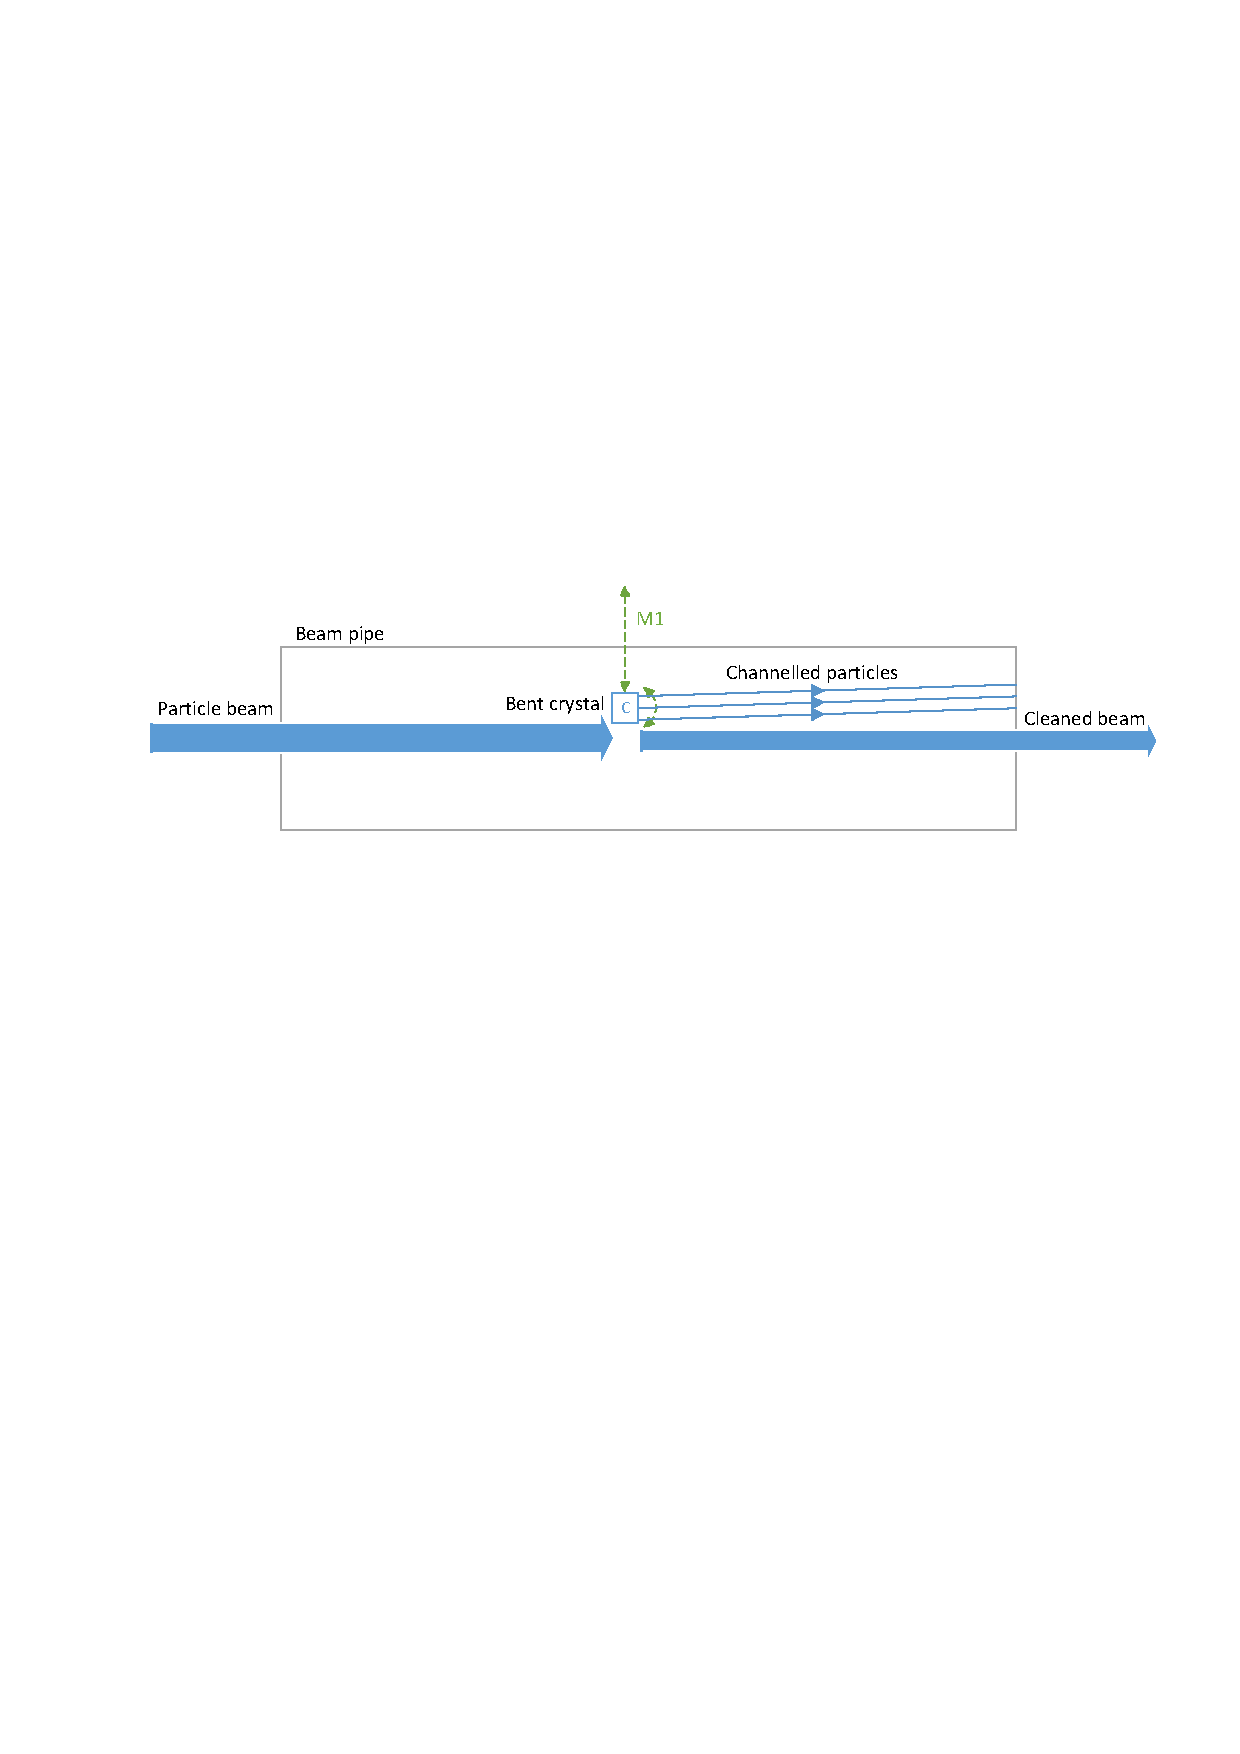
\includegraphics[width=1\textwidth, trim= 2cm 15.5cm 1cm 10cm, clip=true]{../fig/matlab/collimation}
    \caption{\label{fig:collimation}Illustration of the crystal collimation principle.}
  \end{figure}

  Implies in a more efficient cleaning, a less complex system and a reduction of the machine impedance.
\end{frame}

\begin{frame}[fragile]{Purpose and Goal}
  The \textbf{ higher the energy} of the particle the \textbf{lower the angular acceptance} for channeling.
  \begin{itemize}
    \item have a total range of \unit{20}{\milli\rad}
    \item be able to track reference trajectories at ramp rates of \unit{100}{\micro\radianpersecond}
    \item reject external disturbances to maintain a maximum tracking error of $\pm$\unit{1}{\micro\rad} even when the linear axis is moving
  \end{itemize}
\end{frame}

\begin{frame}[fragile]{Challenges}
  \begin{itemize}
    \item Nonlinear effect such as hysteresis and creep
    \item Highly resonant structure
    \item The linear movement adds additional perturbation
    \item System changes due to rotational and linear position, moving center of rotation.
  \end{itemize}
\end{frame}

\begin{frame}[fragile]{Method}
  \begin{itemize}
    \item Literature study
    \item Further investigation of selected control approaches
    \item Benchmarking tests of selected control approaches in simulations
    \item Implementation of the most promising approach
    \item Proposal of controller
  \end{itemize}
\end{frame}

\section{System Overview}

\begin{frame}[fragile]{Crystal Collimator}
  \begin{figure}[h]
    \centering %crop: left bottom right top
    \subfloat[][\label{fig:collimator-side}Side view]{
    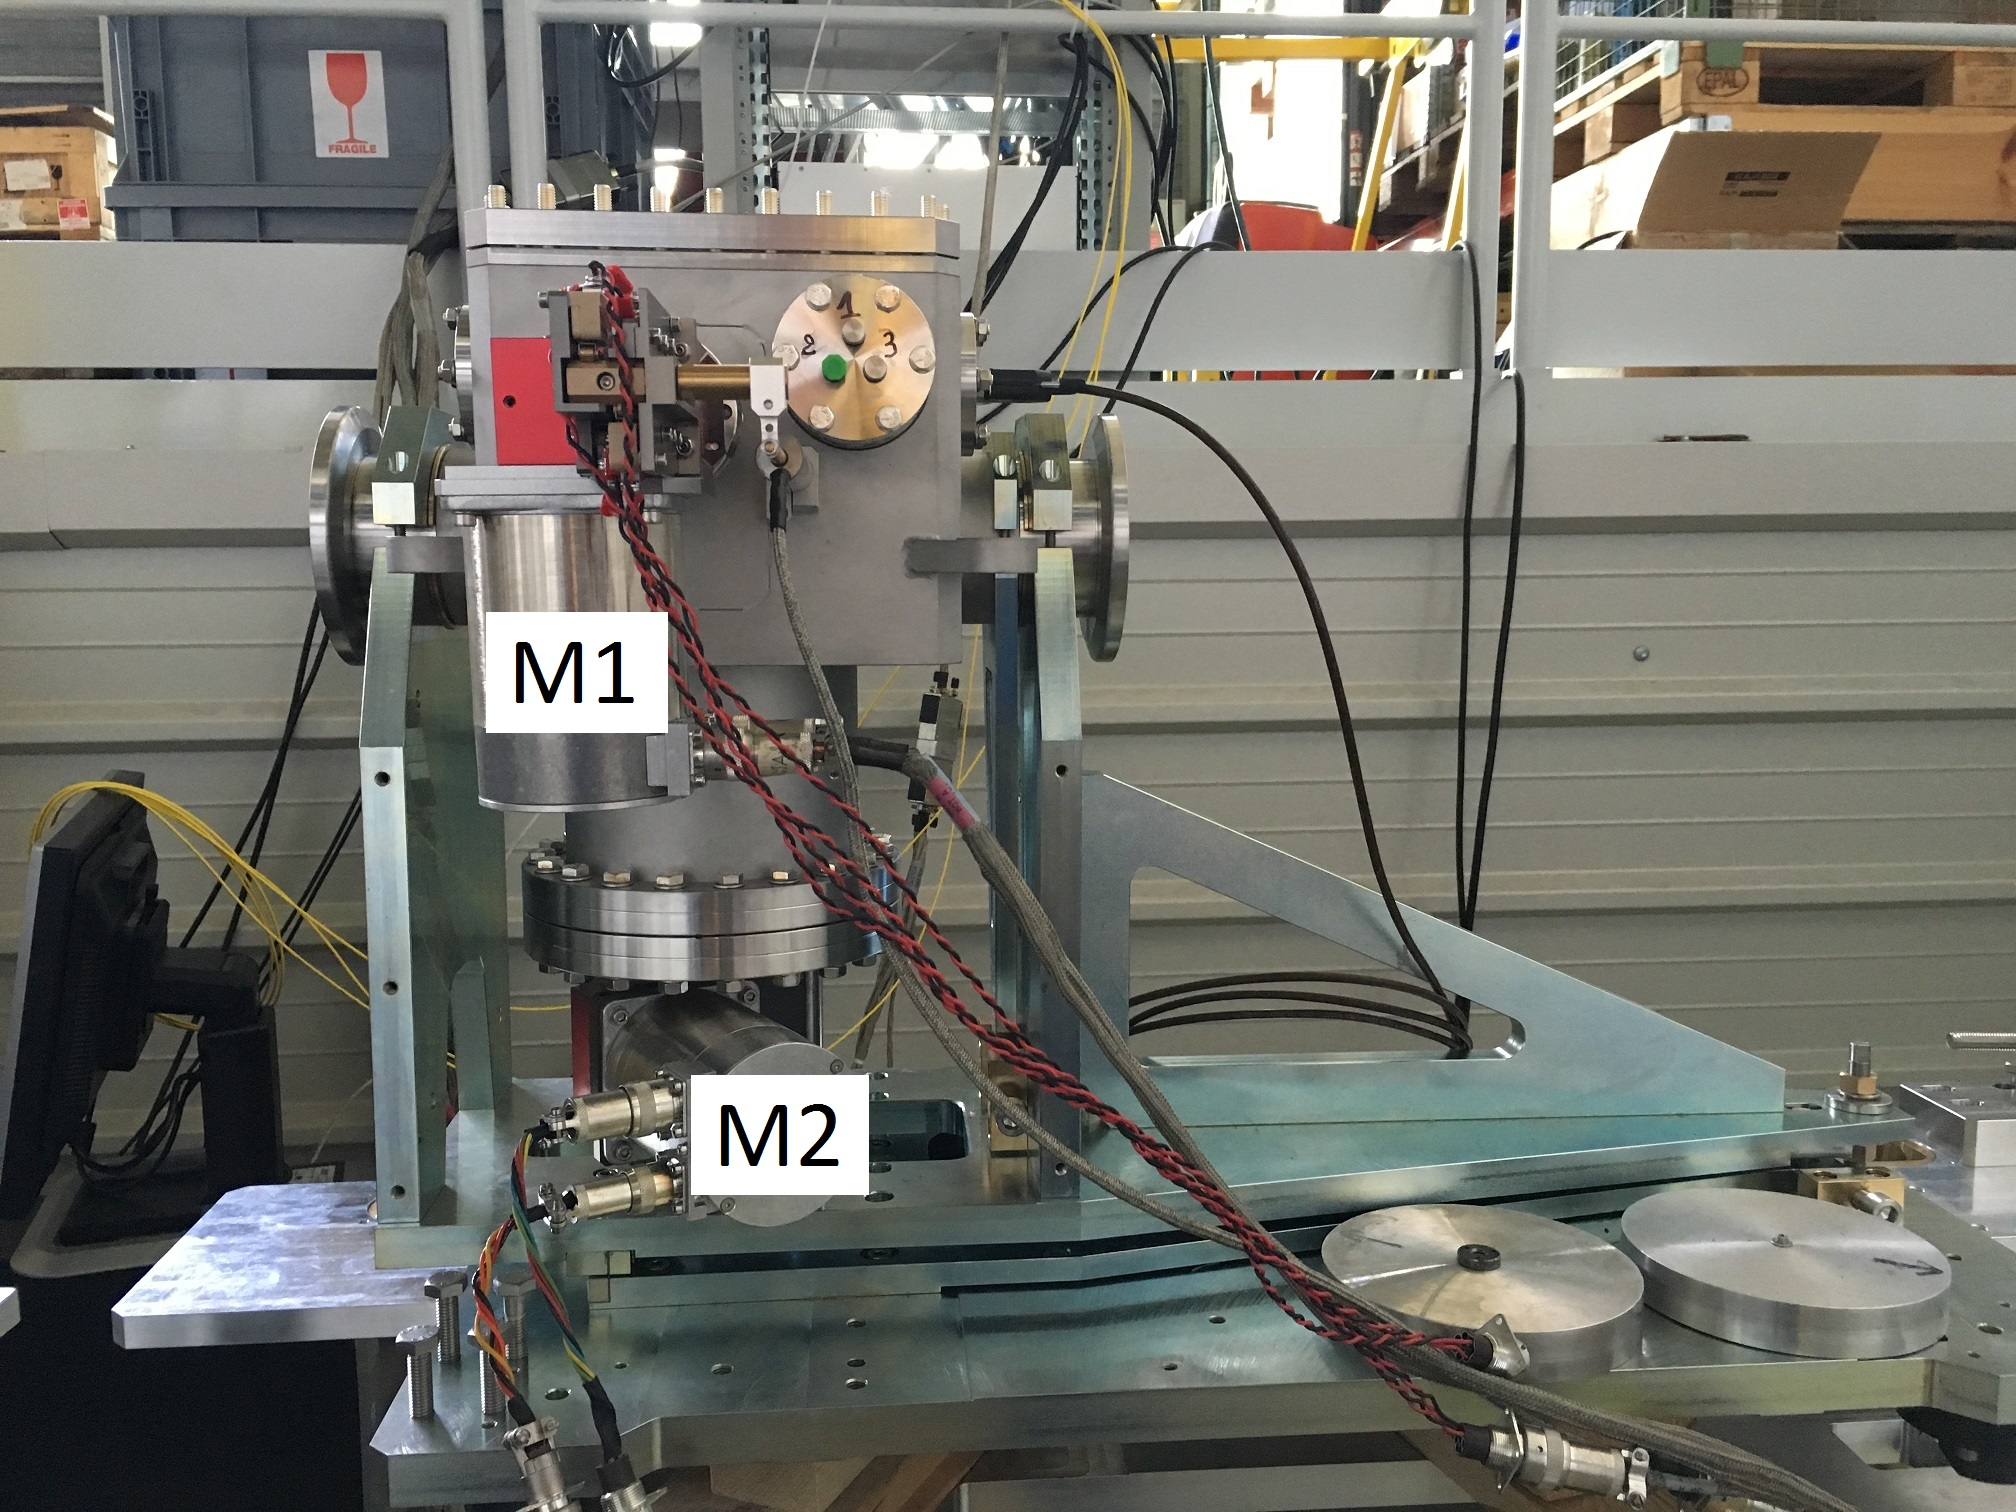
\includegraphics[width=0.4\textwidth, trim=2cm 11cm 2cm 5cm, clip=true]{../fig/collimator-side}}
    \qquad
    \subfloat[][\label{fig:collimator-top}Top view]{
    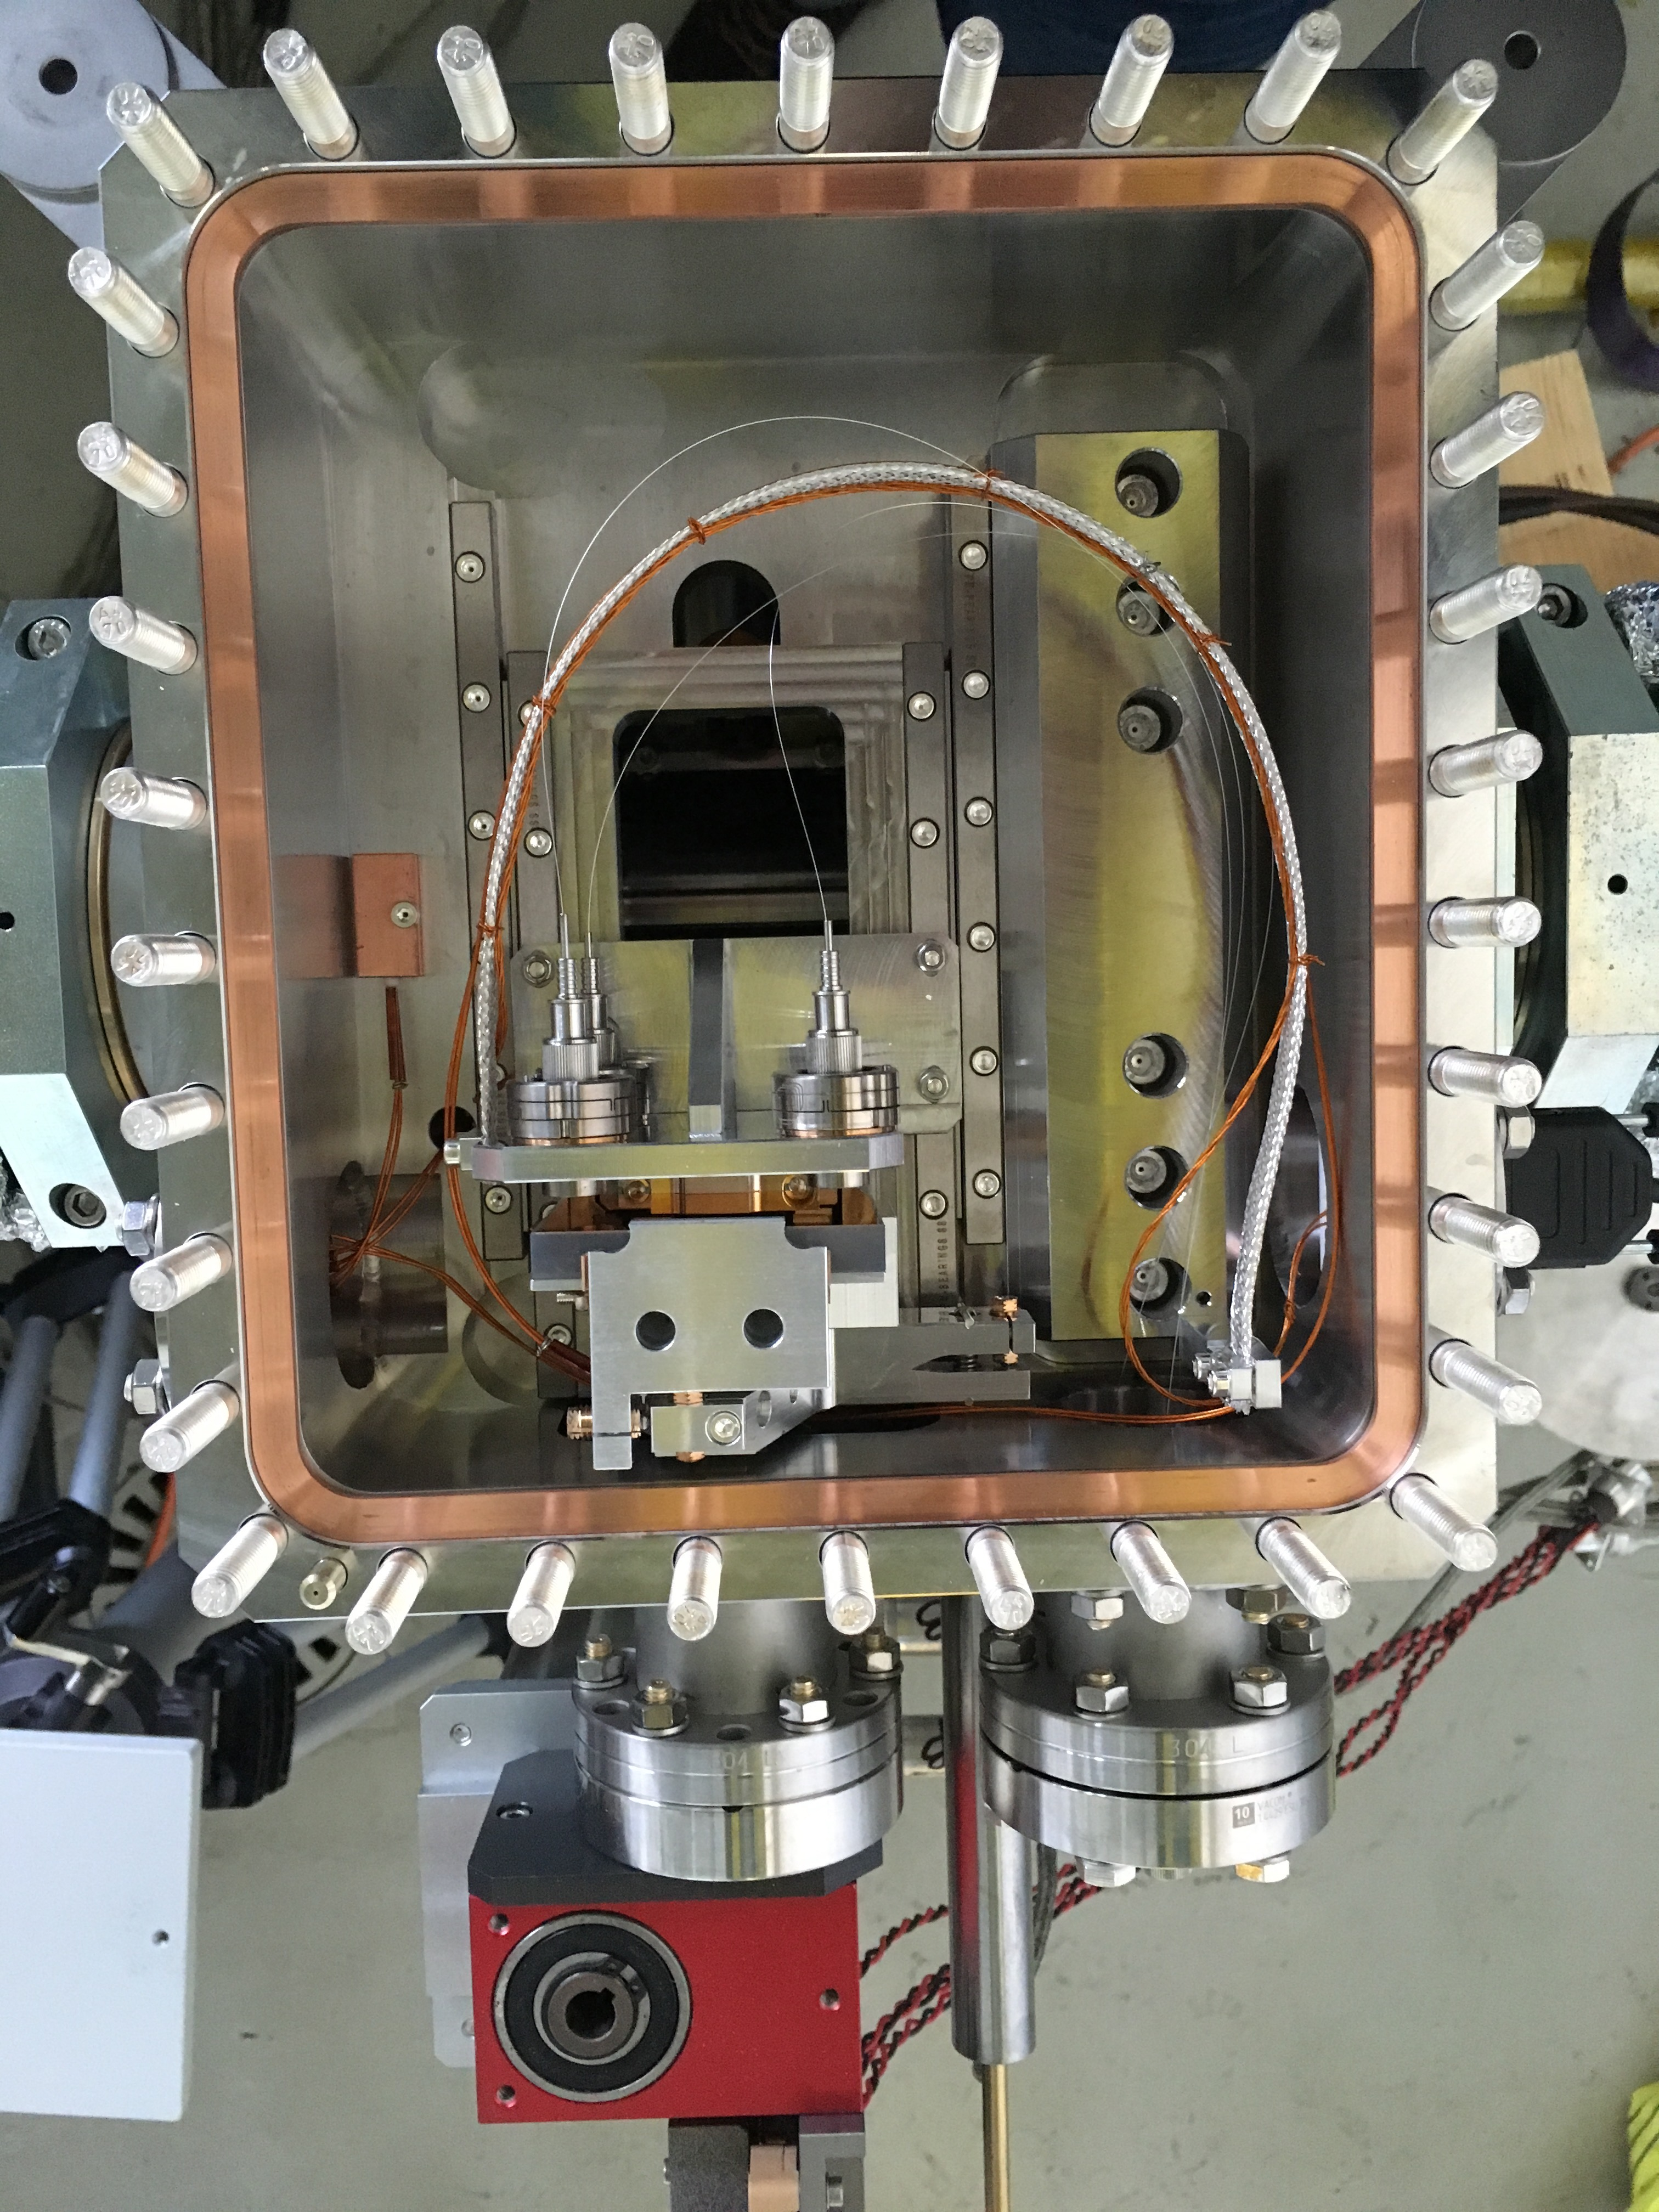
\includegraphics[width=0.4\textwidth, trim=0cm 0cm 0cm 0cm, clip=true]{../fig/collimator-top}}
    \caption{\label{fig:collimator} The new collimator from the side (a) and the top (b).}
  \end{figure}
\end{frame}

\begin{frame}[fragile]{Crystal Collimator}
  \begin{figure}[h!]
    \centering %crop: left bottom right top
    \subfloat[][\label{fig:collimator-through} Giving access]{
    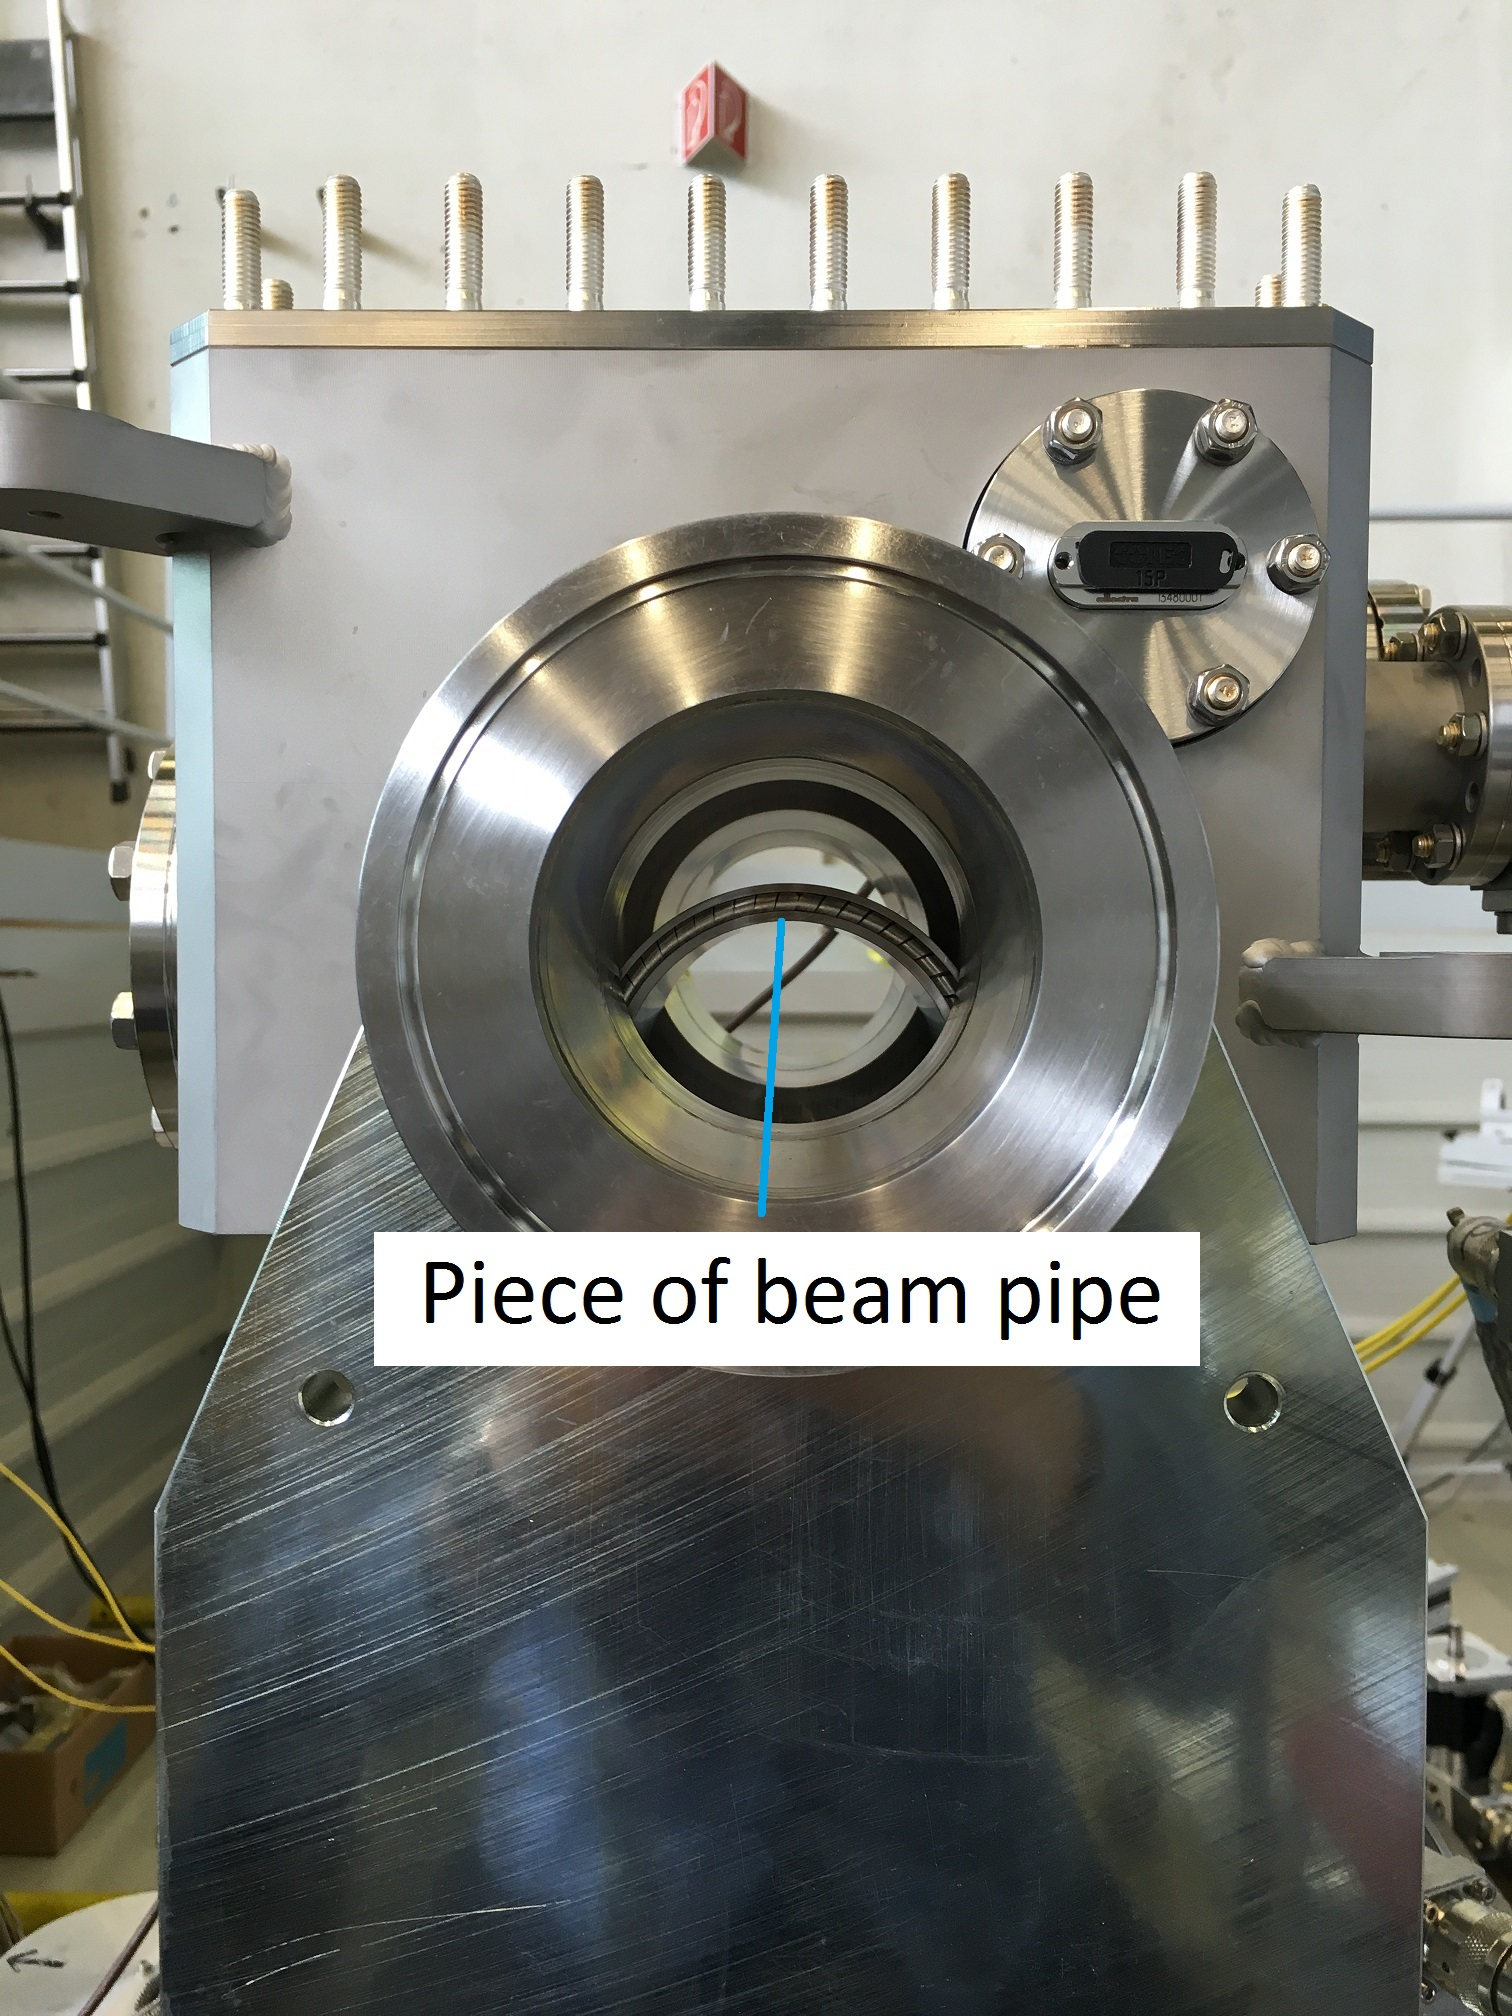
\includegraphics[width=0.4\textwidth, trim=3cm 12.8cm 2cm 5cm, clip=true]{../fig/collimator-through}}
    \qquad
    \subfloat[][\label{fig:collimator-mirror} Insertion of crystal]{
    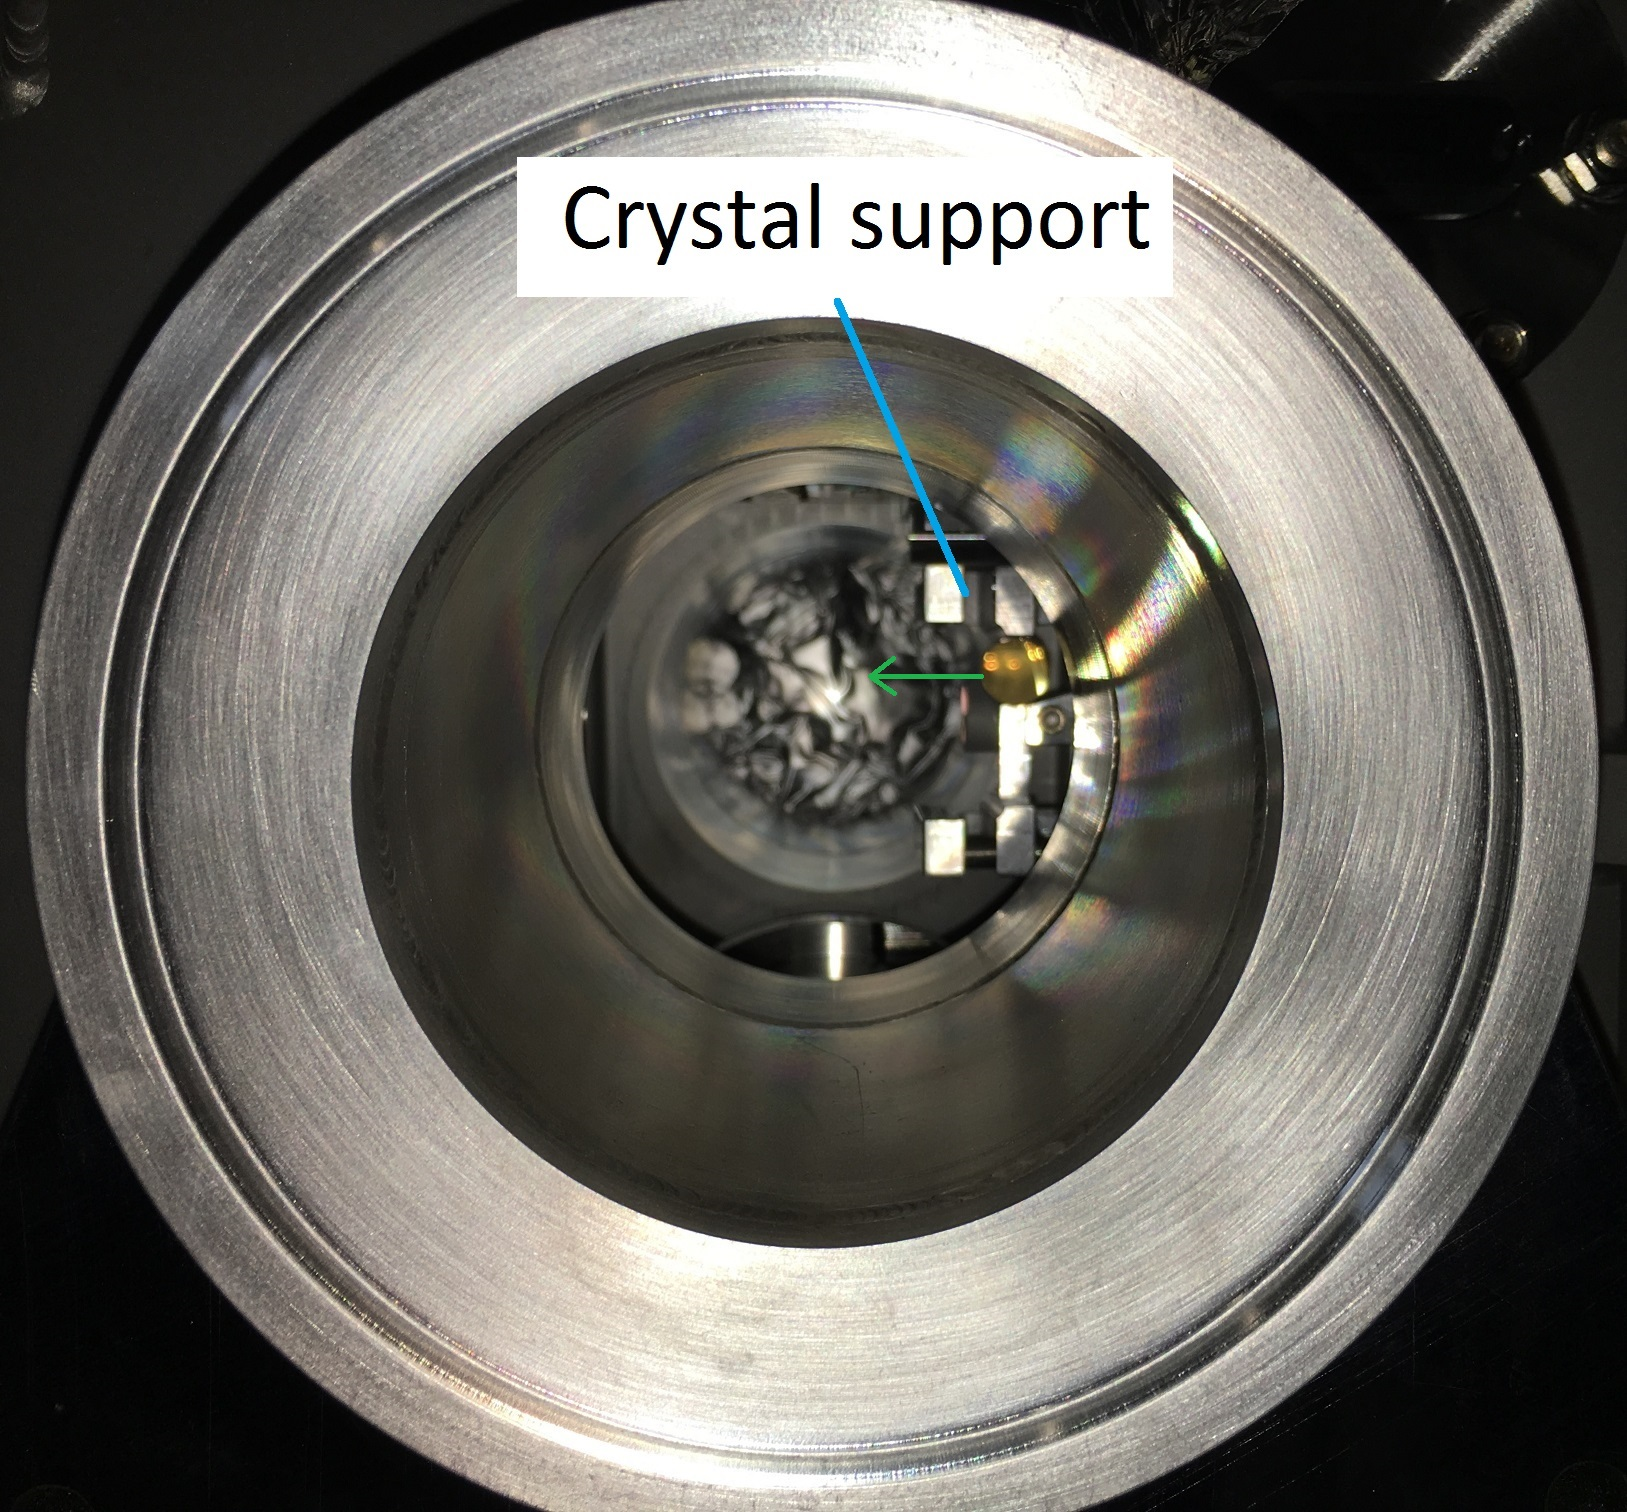
\includegraphics[width=0.4\textwidth, trim=0cm 0cm 0cm 0cm, clip=true]{../fig/collimator-mirror}}
    \caption{\label{fig:collimator-t} The new collimator with the beam pipe piece half-way out (a) and the crystal inserted into the beam pipe (b).}
  \end{figure}
\end{frame}

\begin{frame}{Rotational Stage}
   Displacement: 0 to \unit{30}{\micro\meter} (-20 and +150 V) $\implies$ 0 to 20 mrad.
  \begin{figure}[h]
    \centering
    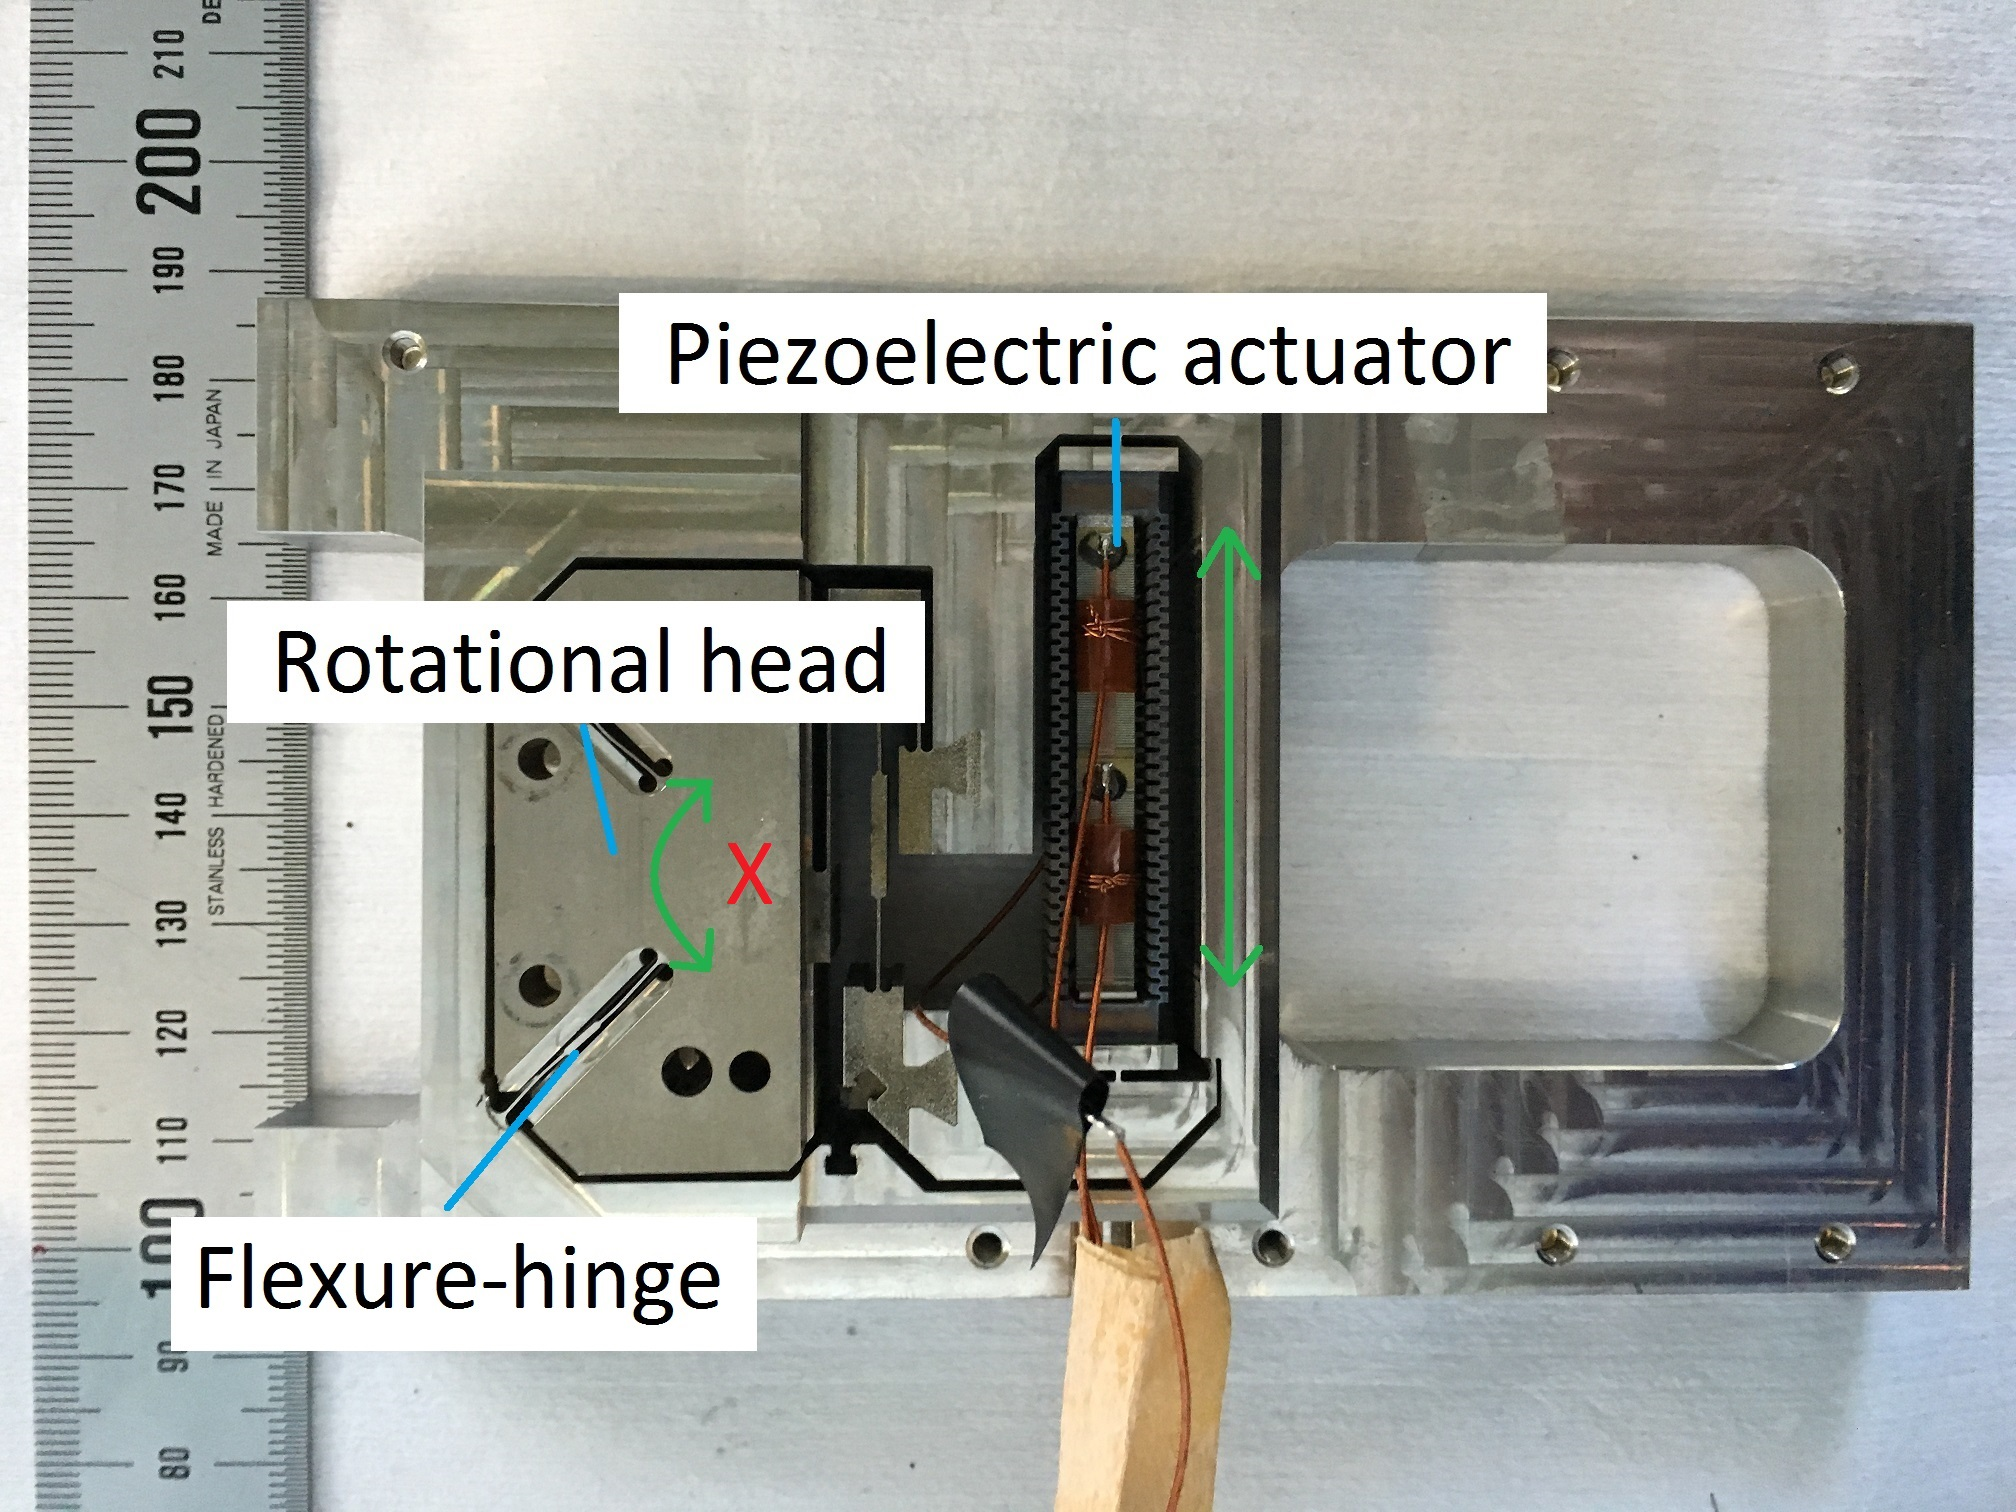
\includegraphics[width=0.7\textwidth]{../fig/rotational-stage.jpg}
    \caption{\label{fig:rotationalstage} Piezo-actuated rotational stage used in the new collimator.}
  \end{figure}
\end{frame}

\begin{frame}{Rotational Stage}
  \begin{figure}[h]
    \centering
    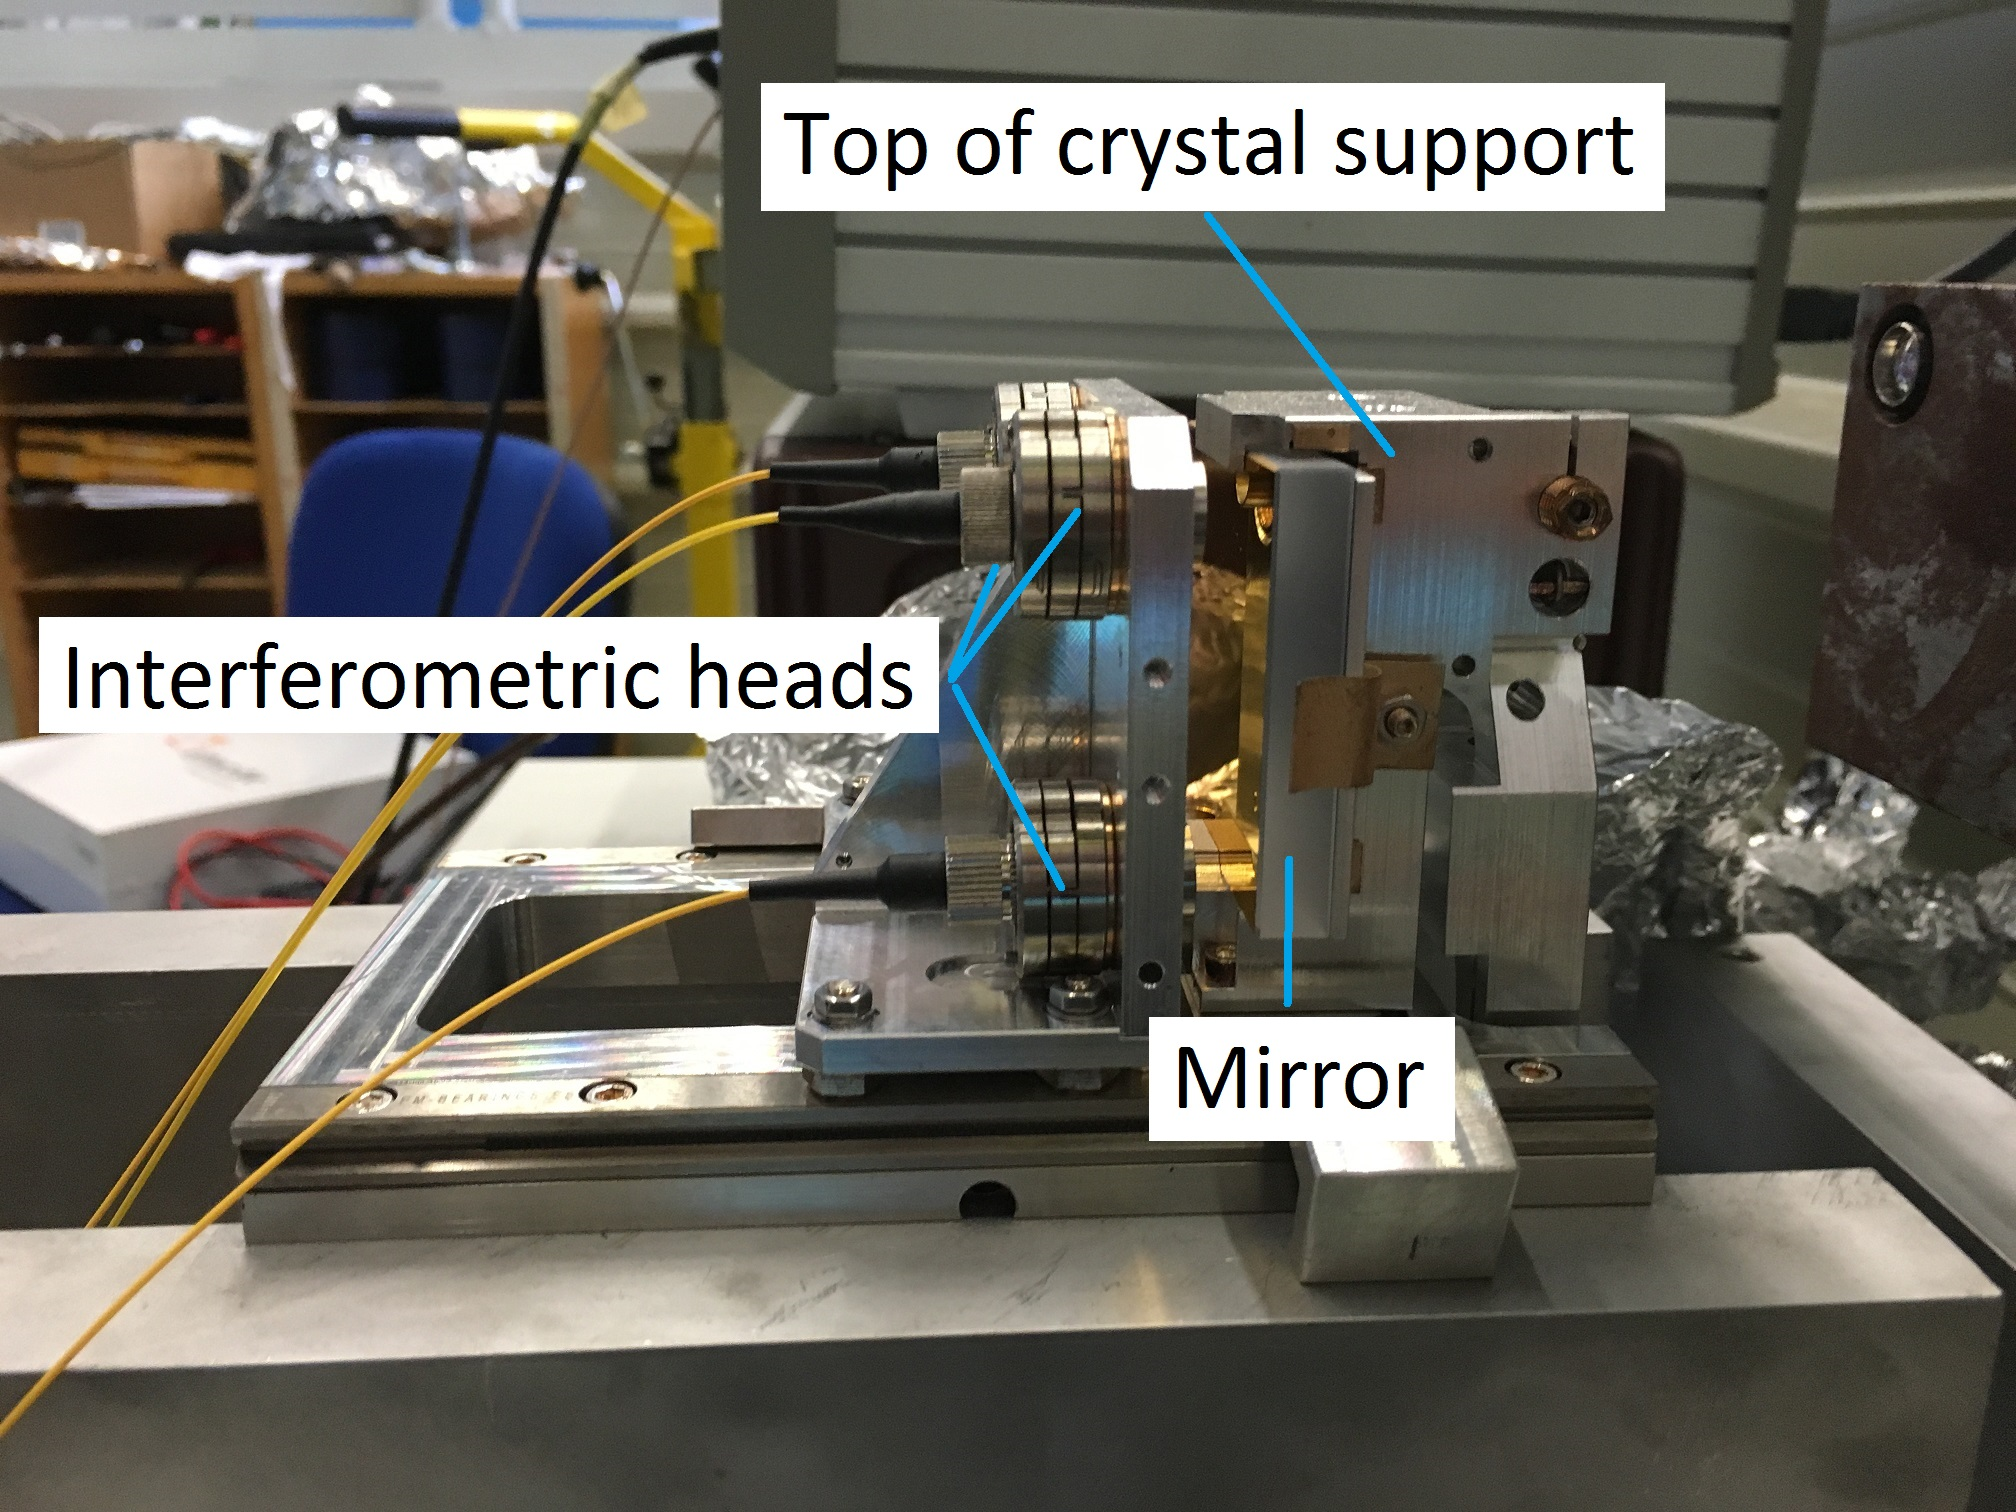
\includegraphics[width=0.7\textwidth]{../fig/rotational-stage-interferometer.jpg}
    \caption{\label{fig:rotationalstage-side} Rotational stage with the crystal support and the interferometric system mounted on top.}
  \end{figure}
\end{frame}

\begin{frame}{Piezoelectric stack actuators}
  \begin{itemize}
    \item Piezoelectric effect
    \item Many thin electro-active ceramic disks connected in parallel
    \item Provides high stiffness and long displacement ranges
    \item Nonlinear effects
  \end{itemize}

  \begin{figure}[h!]
    \centering %crop: left bottom right top
    \subfloat[][\label{fig:hysteresis} Hysteresis loop]{
    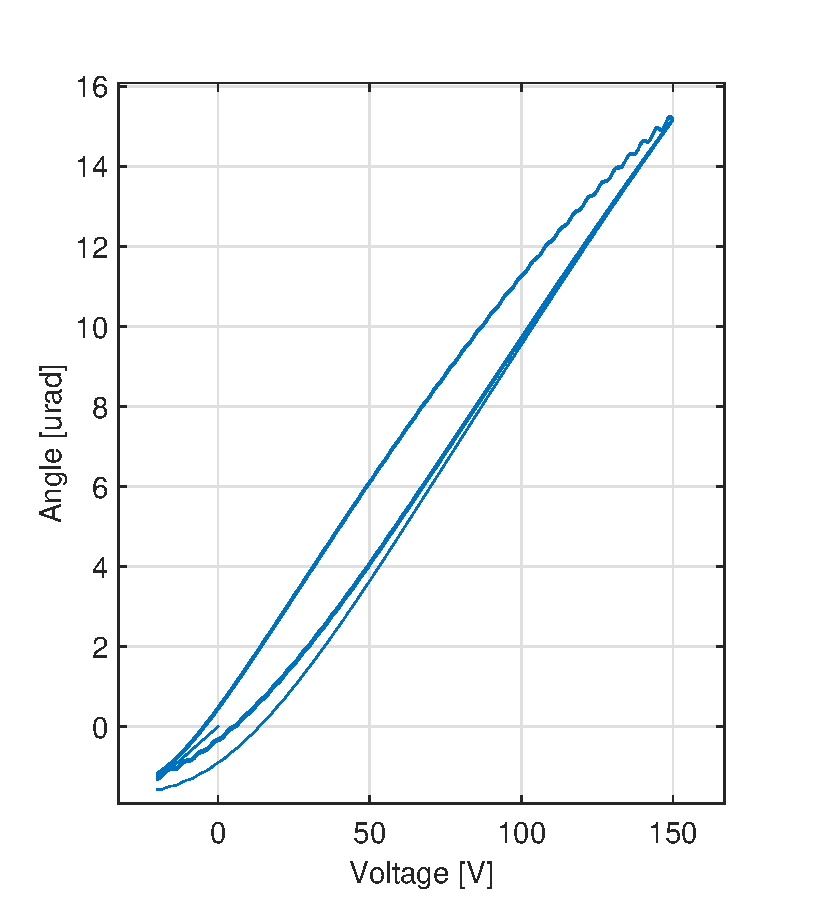
\includegraphics[width=0.3\textwidth, trim=0cm 0cm 1cm 0cm, clip=true]{../fig/matlab/hysteresis.eps}}
    \qquad
    \subfloat[][\label{fig:creep} Creep effect]{
    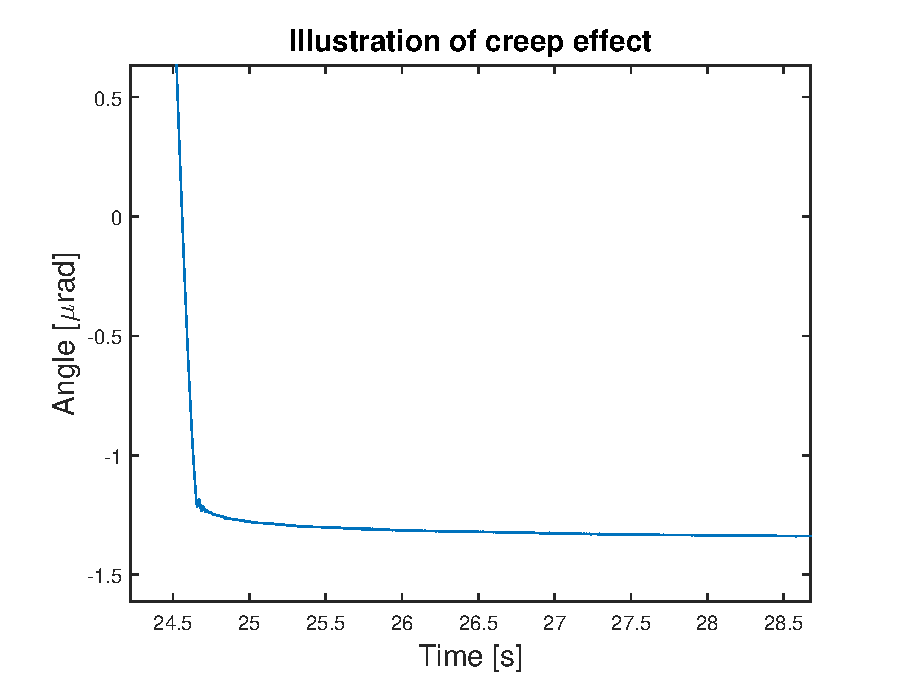
\includegraphics[width=0.3\textwidth, trim=0cm 0cm 1cm 0cm, clip=true]{../fig/matlab/creep.eps}}
    \caption{\label{fig:effects} Illustration of the hysteresis effect (a) and creep effect (b).}
  \end{figure}
\end{frame}

\begin{frame}{Modeling}
  \begin{itemize}
    \item \alert{Hysteresis effect} - Modeled by a Maxwell slip model
    \item \alert{Creep effect} - Efficiently eliminated in closed loop
    \item \alert{Rotational stage} - modeled as a Hammerstein structure
  \end{itemize}
  \begin{figure}[h]
    \centering %crop: left bottom right top
    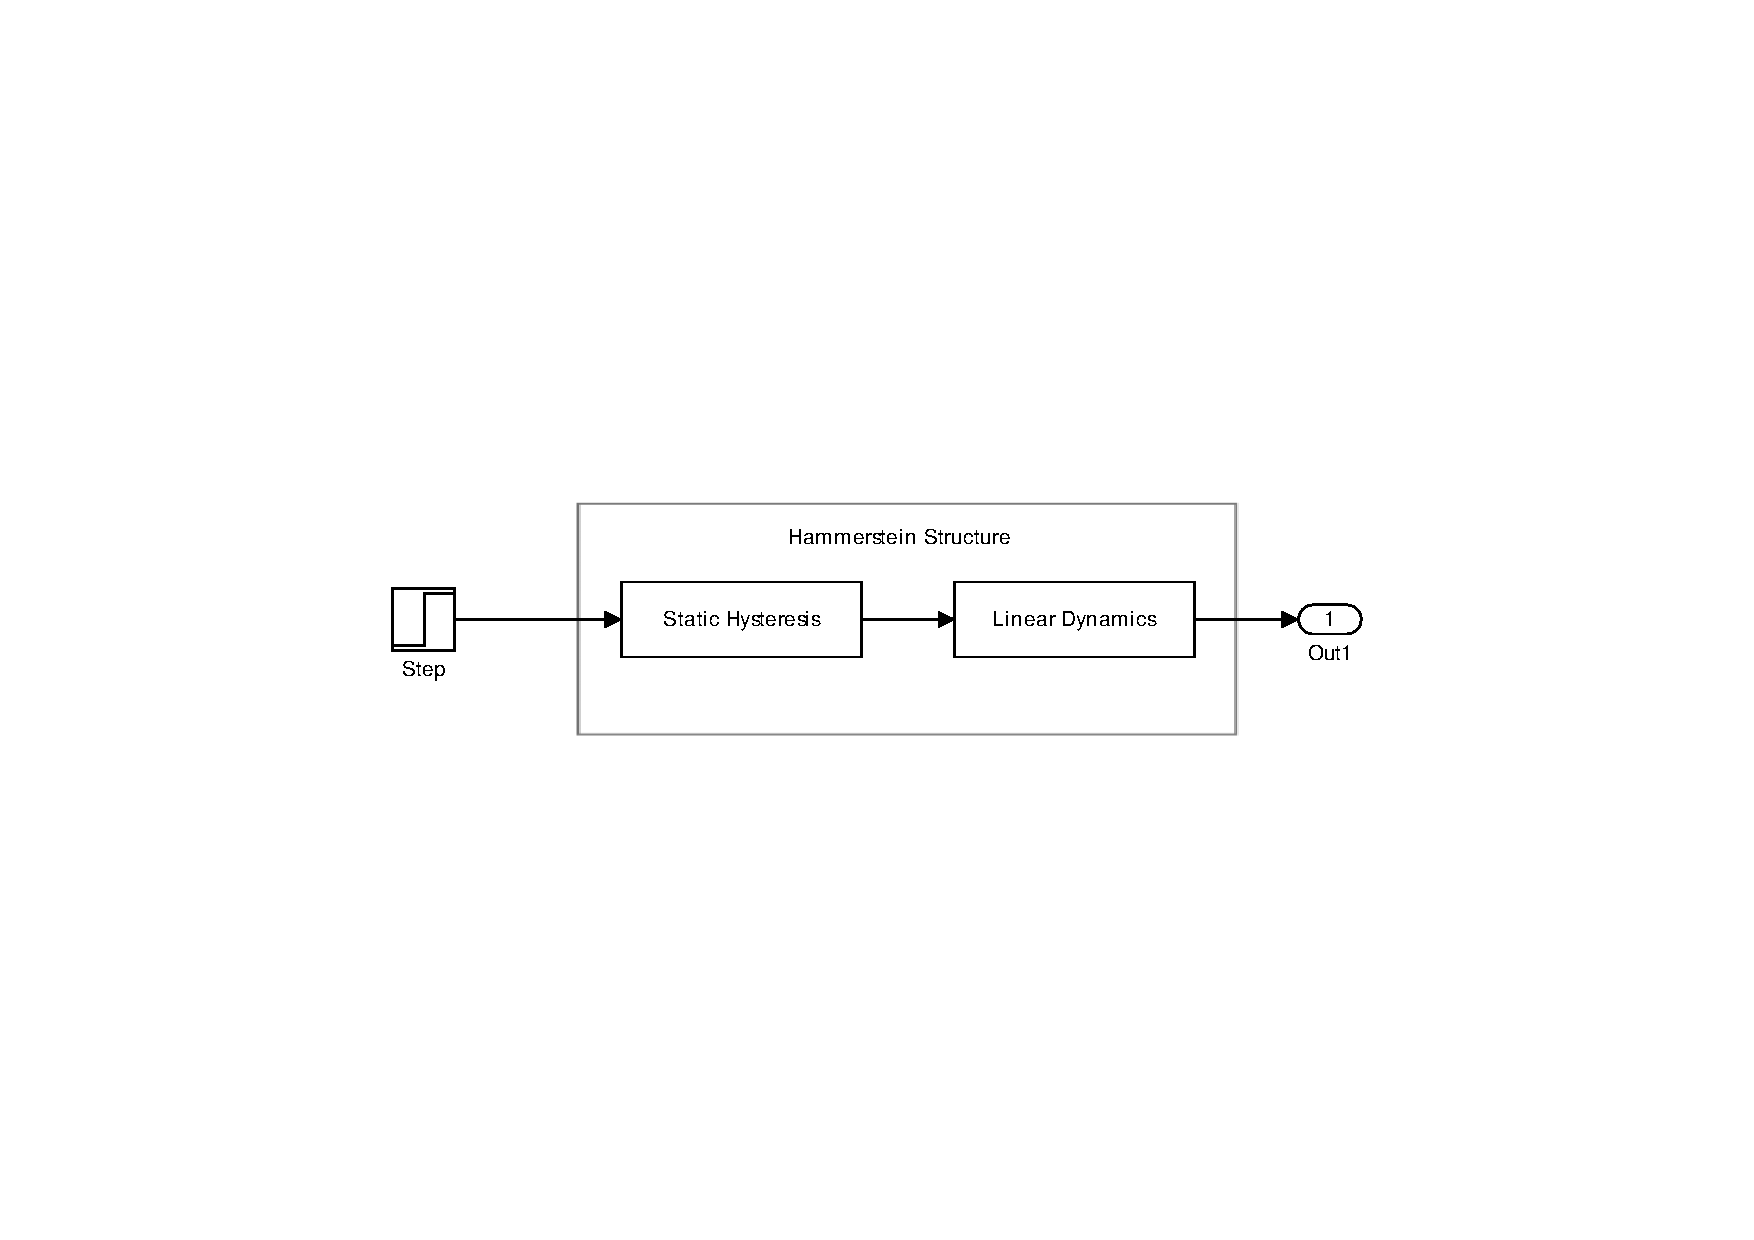
\includegraphics[width=0.7\textwidth, trim=8cm 8cm 7.73cm 8cm, clip=true]{../fig/matlab/hammerstein}
    \caption{\label{fig:hammerstein}Block diagram of a Hammerstein structure, consisting of two blocks in series, modeling the static hysteresis and the linear dynamics, respectively.}
  \end{figure}
\end{frame}

\begin{frame}{Linear System Identification}
  \begin{figure}[h!]
    \centering
    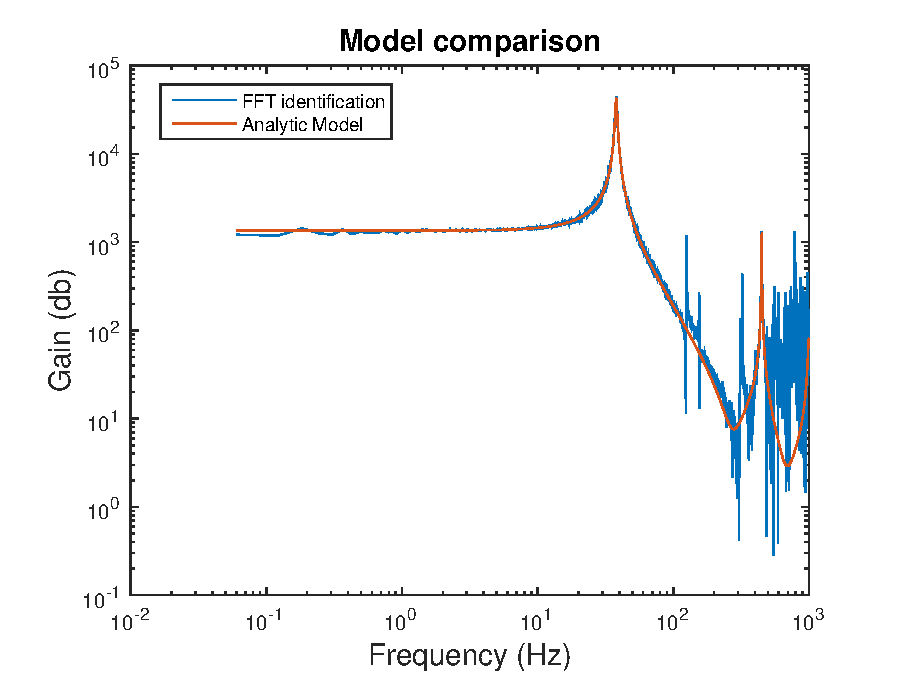
\includegraphics[width=0.7\textwidth]{../fig/matlab/model.eps}
    \caption{\label{fig:model} Model fit of the system model with 5 zeros and 6 poles to the \textsc{FFT} of the acquired data.}
  \end{figure}
\end{frame}

\begin{frame}{Linear System Identification}
  \begin{figure}[h]
    \centering %crop: left bottom right top
    \subfloat[][\label{fig:different_angles}Different rotational head positions]{
    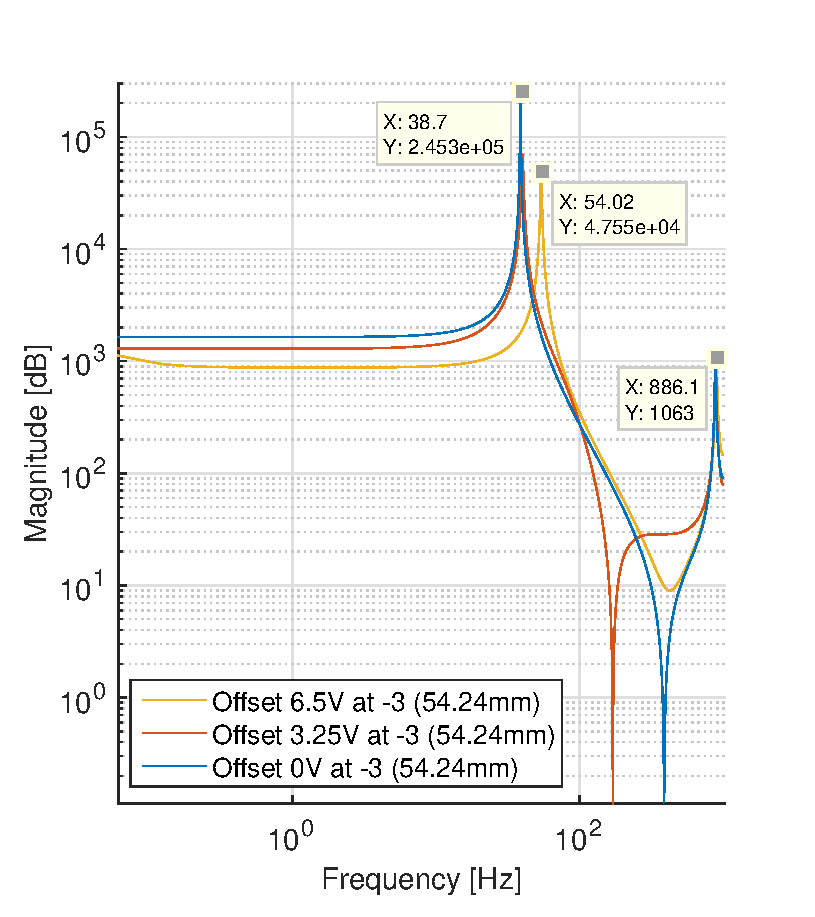
\includegraphics[width=0.4\textwidth, trim=0cm 0cm 0.8cm 1cm, clip=true]{../fig/matlab/modelcomparison_diffvolt2.eps}}
    \qquad
    \subfloat[][\label{fig:different_lin_pos}Different linear axis positions]{
    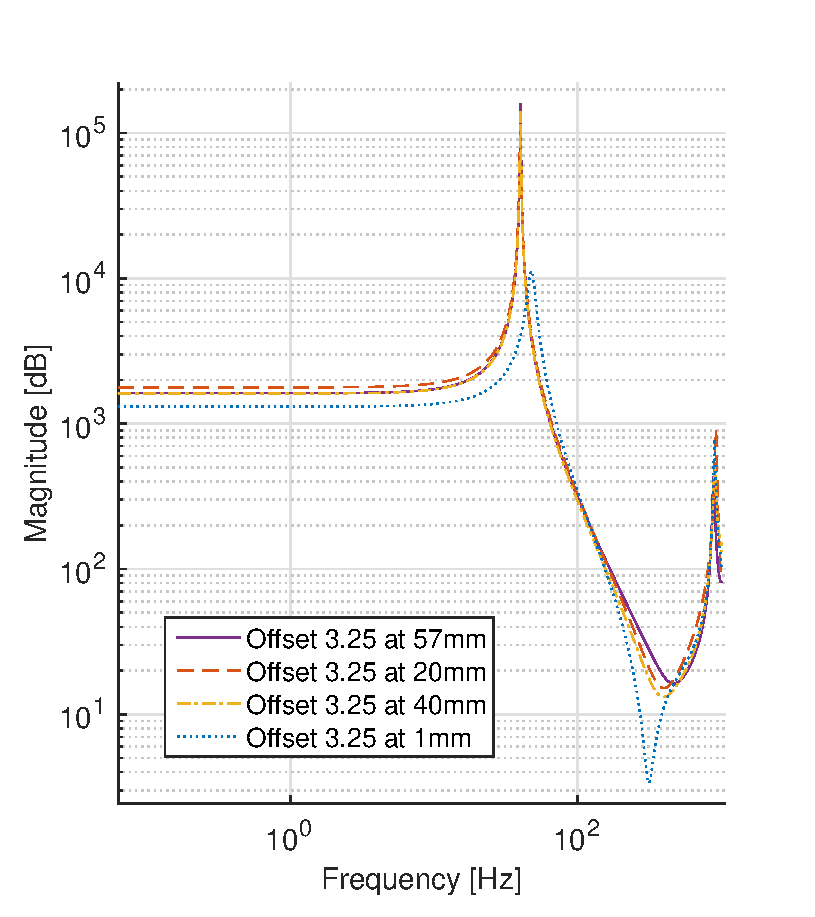
\includegraphics[width=0.4\textwidth, trim=0cm 0cm 0.8cm 1cm, clip=true]{../fig/matlab/modelcomparison2.eps}}
    \caption{\label{fig:different_lin_angle} Identified models with different rotational positions (linear axis in 54.24 mm) is shown in (a) and with different linear axis positions (rotational position corresponding to 3.25 V) is shown in (b).}
  \end{figure}
\end{frame}

\begin{frame}{Present Control Approach}
  \begin{equation*}
    e = \lim_{n\to \infty} \left(1 + \frac{1}{n}\right)^n
  \end{equation*}
\end{frame}

\section{Approaches and Simulation Results}

\begin{frame}{Integral Resonance Control}
\end{frame}

\begin{frame}{Model Reference Adaptive Controller}
\end{frame}

\begin{frame}{Harmonic Cancellation}
\end{frame}

\begin{frame}{Comparison}
\end{frame}

\section{Implementation}

\begin{frame}{Setup}
\end{frame}

\begin{frame}{Experimental Results}
\end{frame}


\section{Conclusion}

\begin{frame}{Simulation Results}
\end{frame}

\begin{frame}{Experimental Results}
\end{frame}

\begin{frame}{Summary}
\end{frame}

\begin{frame}[standout]
  Questions?
\end{frame}

\appendix

\begin{frame}[allowframebreaks]{References}

  \bibliography{pres}
  \bibliographystyle{abbrv}

\end{frame}

\end{document}
